\section{Empirical Study}\label{Sec:empirical}
\subsection{Data description: Soichi}
\begin{itemize}
	\item Data description
\end{itemize}

\\

\\

We use the Freedom House Political Right Index as one of proxies of political right. It has researched since 1950 and now researches 209 countries and territories. It measures how countries has ideal democratic political situation and a country gets highest score, which is 1, if it has ideal political situation for democracy. Worst score is 7 and it means it is least free in terms democracy nation. For each country and territory, Freedom in the World analyzes the electoral process, political pluralism and participation, the functioning of the government, freedom of expression and of belief, associational and organizational rights, the rule of law, and personal autonomy and individual rights. Also, because Freedom House index changed the way of the estimation in 1972, we use 1972 data for 1970, and scattering pattern has been changed from before ones before and after 1965.  To enhance accuracy of our estimation, we use supplement index with the related variables from Kenneth A. Bollen (1990, 2001) for 1950 to 1965 data.


We also introduce PolityI\hspace{-.1em}V political right index. PolityI\hspace{-.1em}V estimate the level of each country’s democracy by the competitiveness of political participation, the competitiveness of executive recruitment, the openness of executive recruitment, and the constraints on the chief executive. If the country has best democratic political situation, it is scored 10, the maximum points. Worst score means autocracy and scores 0. Since this proxy has long term data which is from 1800 to recent data, we can analyze before the World War Second through this data set. To compare both two proxies, we normalize them between 0 to 1, and o is worst situation for democracy, and 1 means best political situation for democracy. 


GDP per capita data for post war period are from Ala Heston, Robert Summers, and Bettina Atten (2002) and GDP per capita(in contrast 1990 dollars) for the longer sample are from Maddison (2003).


We prepare three data sets from "Income and Democracy"(2008) data set which is written by Daron Acemoglu, Simon Johnson, James A. Robinson, and Pierre Yared in American Economic Association.

Table1 describe three main variables. The sample period is 1960-2000, and each observations have 5 years interval. High-income countries and low income countries in Table1 are splited by median of income data.

Figure.1 plots income and Freedom House Index data of each county. We use so much samples in a graph. Thus, we set "G" groups to reduce the number of plots in the graph. Each country in same group has similar combination of log GDP per capita and Freedom House Political Right Index. G01 is Angola and Mauritania; G02 is Nigeria and Chad; G03 is Kenya and Cambodia; G04 is Algeria and Lebanon; G05 is Burkina Faso, Niger, and Yemen; G06 is Gabon and Malaysia; G07 is Dominica Republic and Slovenia; G08 is Brazil and Venezuela; G09 is Botswana, Dominica, Poland, and St. Vincent and the Grenadines; G10 is Hungry and Uruguay; G11 is Costa Rica and Grenada; G12 is Belize and St. Lucia; G13 is St. Kitts and Nevis and Trinidad and Tobago; G14 is Greece and Malta; G15 is Barbados, Cyprus, Spain , and Portugal; G16 is Finland, United Kingdom, Ireland, and New Zealand; G17 is Australia, Austria, Belgium, Canada, Germany, Denmark, France, Israel, Italia, Netherland, Norway, and Sweden; and G18 is Switzerland and USA. According to this figure, countries which has large GDP per capita tend to have good score of Freedom House Index through one of the latest data.


Figure.2 and 3 show the outline of change of each country’s data. Vertical axis means changes from 1975 to 1995 of Freedom house index in Figure2 and PolityI\hspace{-.1em}V in Figure.3, and horizontal axis is Change in log GDP per capita. The "G" prefix corresponds to the average for groups of countries. G01 is Fiji and Kenya; G02 is Colombia and India; G03 is Iran, Jamaica, and Slovakia; G04 is Chile and Dominica Republic; G05 is Cote d’Ivoire and Rwanda; G06 is Switzerland, Costa Rica, and New Zealand; G07 is Algeria and Sweden; G08 is Australia, Denmark, Morocco, and Netherland; G09 is Belgium, Canada, France, and United Kingdom; G10 is Austria, Egypt, Iceland, Italia, Paraguay, and USA; G11 is Barbados, Norway, and Tunisia; G121 is Ireland and Syrian Arab Republic; G13 is Burundi and Tanzania; G14 is Gabon, Mexico, and Trinidad and Tobago; G15 is Peru and Senegal; G16 is Haiti and Jordan; G17 is Lesotho and Nepal; G18 is Brazil and Congo Republic; G19 is Argelia and Honduras; G20 is Benin and Mali; G21 is Greece, Malawi, and Panama; and G22 is Ecuador and Hungry.


For Figure3, G01 is Switzerland, Costa Rica, and New Zealand; G02 is Australia, Denmark, and Netherland; G03 is Belgium, Canada, Finland, United Kingdom, and Turkey; G04 is Austria, Colombia, IND, Iceland, Israel, Italia, and USA; G05 is Ireland and Syria; G06 is Kenya, Morocco, and Uruguay; G07 is Bolivia and Mali; G08 is Malawi and Panama; G09 is Greece and Lesotho; and G10 is Brazil and Spain. 


Through these figures, we can say that in terms Freedom House Index, expansion of GDP per capita shows positive relation between democracy score, on the other hand in terms of PolityI\hspace{-.1em}V, it shows negative. However, plots in both figures are dispersed and degree of positive and negative relation is little.


Figure.4 is a scatter diagram of panel data for each 5 year from 1950 to 2000. Vertical axis is Freedom House Index and horizontal axis shows income per capita. Blue line in each graph is standard regression line of freedom house index and income of each country. Independent variable is Freedom House index and dependent variable is Log GDP per capita. Each year data always shows countries which has large log GDP per capita has get good score of Freedom House Political Right Index. 

\begin{center}
	\includegraphics[width=15cm]{f1 fixed.png}
\end{center}
}
\begin{center}
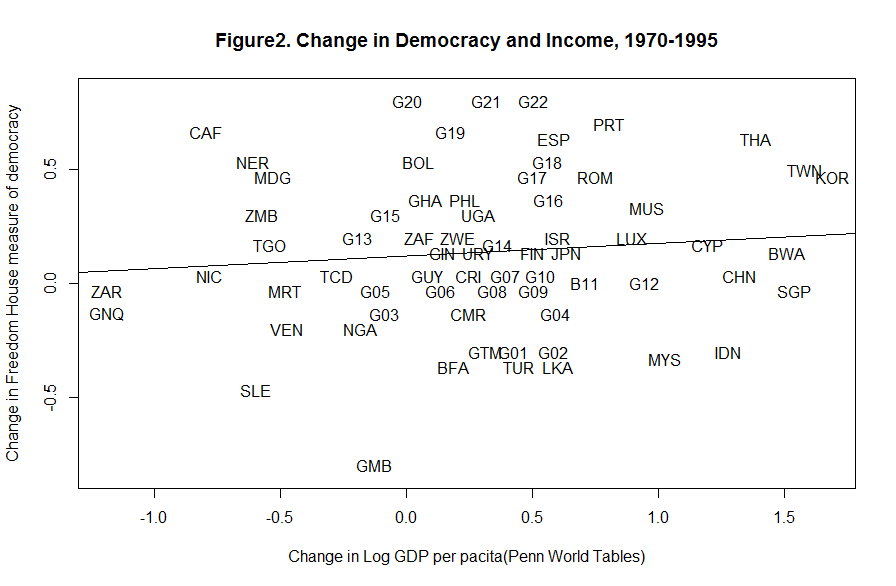
\includegraphics[width=15cm]{f2 fixed.png}
\end{center}
}
\begin{center}
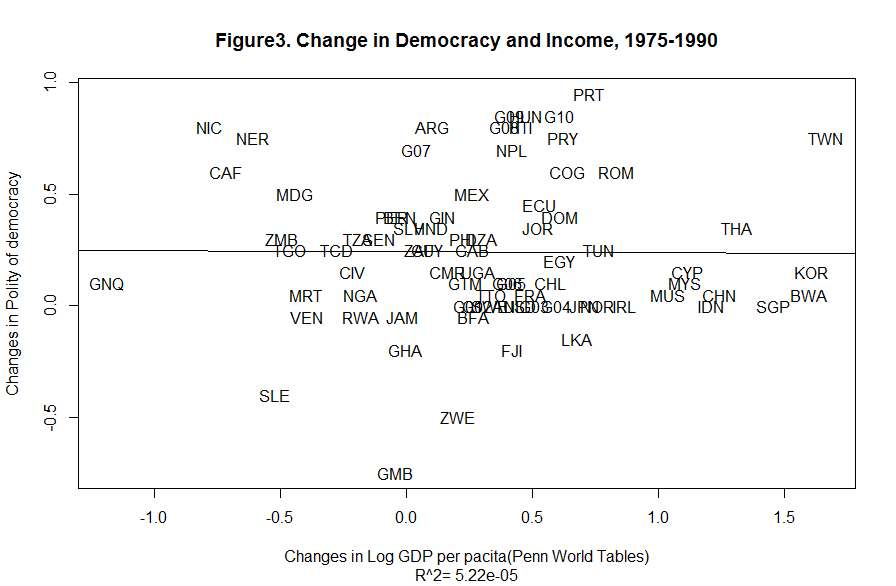
\includegraphics[width=15cm]{Figure3.png}
\end{center}
}


\begin{center}
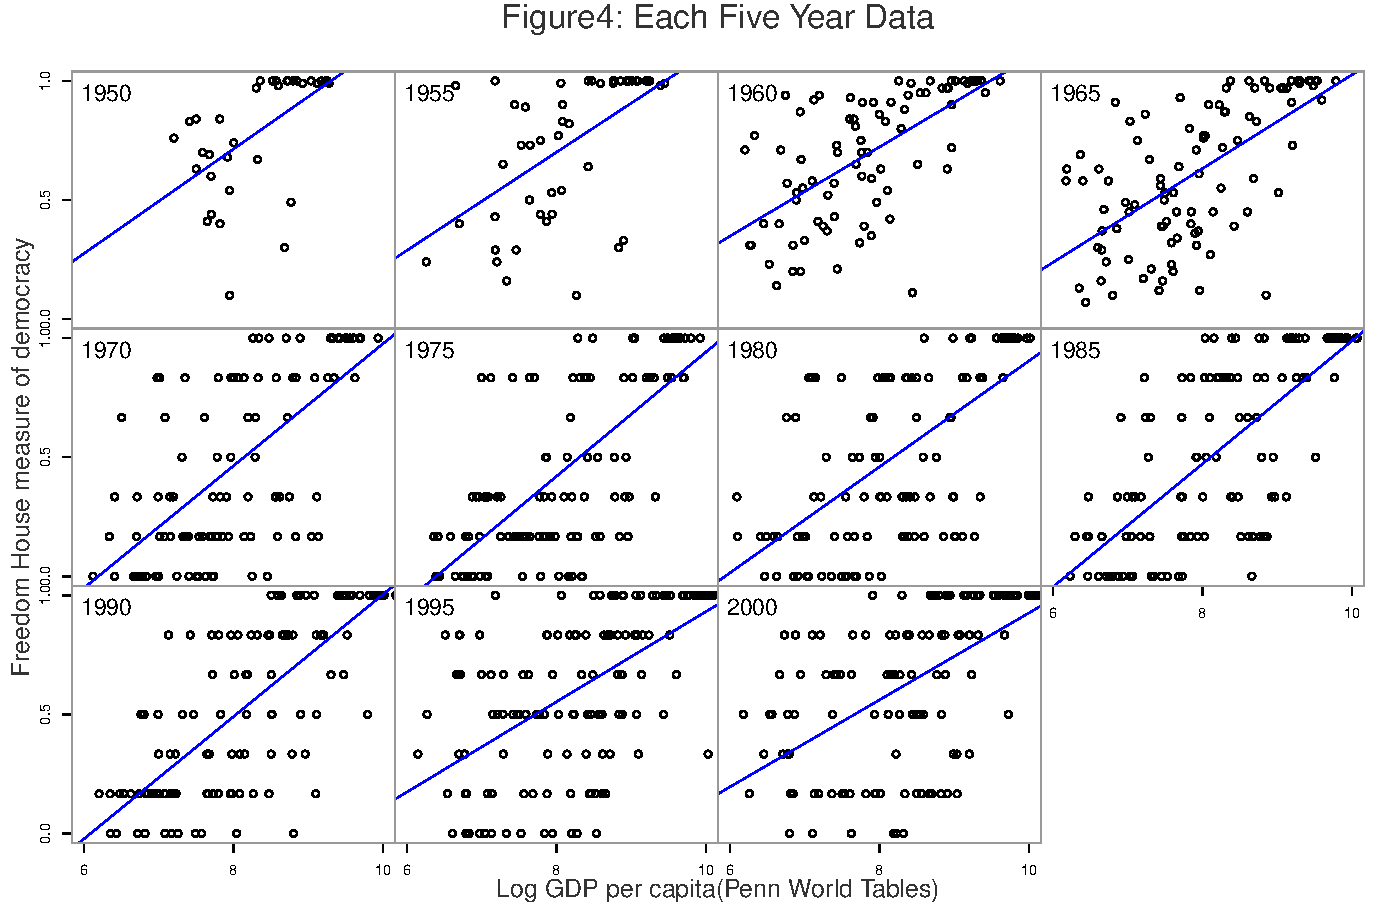
\includegraphics[width=15cm]{F4final.pdf}
\end{center}
}


\subsection{Regression Specification: Hyerin}
\ \ \ In this section, we discuss the causal effect of income on democracy. The relation between democracy scores and income per capita is estimated using the following simple econometric model:  
\begin{align}
d_{i,t} = \alpha d_{i,t-1} + \gamma y_{i,t-1}+ X'_{i,t-1}\beta + \mu_{t}+\delta_{i} + u_{i,t}
\end{align}
\ \ \ \ The democracy score of coutry $i$ in time period $t$ is denoted by $d_{i,t}$. To capture persistency of it, the lagged value of this variable, $d_{i,t}$, is included as a regressor in the model. $y_{i,t-1}$ denotes the lagged value of country $i$'s log income per capita and the estimated coefficient, $\gamma$, measures the causal effect of income per capita on democracy. If an increase in income per capita leads to an higher score of democracy, then the coefficient on the lagged value of log income per capita $\gamma$ should be positive. A full set of coutry dummies and time effects   $\delta_{i}$ $\mu_{t}$. All other potential covariates are denoted in the vector formation,  $X'_{i,t-1}$. To control for country-specific factors a full set of country dummies, $\delta_{i}$, is included in the right-hand side. In addition, to capture common shocks over all sample countries, it introduces $\mu_{t}$ as a full set of time effects. An error term is denoted as $u_{i,t}$.\\


\subsection{Regression Estimates}
\subsubsection{Fixed Effects: Soichi}
\\
Table 2 shows result of our estimation. We use 1960-2000 data of Freedom House Index as a proxy of democracy. All standard errors in the paper robust against heteroskedasticity and serial correlation at the country level.\\
First column in Table 2 shows result of our analysis with Standard Pooled OLS which is most typical way of estimate in the recent literature using the five-year data and dependent variable is five-year democracy data and independent variables are lagged five-year democracy and GDP per capita data. These lagged variables function as the country variables and full set of time series dummies. Though the result, lagged democracy and GDP per capita shows highly statistically significant. A coefficient of lagged democracy is 0.706, so we can say it has large effect, however, lagged GDP per capita is only 0.072 with 0.010 standard error. Therefore, in this estimation we can say that an impact of income per capita to democracy is too small and limited to take consider. \\
Other results in Table 2 show results through fixed effect. Colum 2 shows result of fixed effect OLS with same variables with the estimation of column 1. Democracy coefficient is 0.010 and since a standard error is 0.035, this coefficient is statistically insignificant. Thorough this estimation, we can say that the effect of logged GDP per capita disappears if we use fixed effect OLS.  \\
Column 3 shows a result of more simple model. In this model, we estimate a model of which independent variable is only lagged GDP per capita with fixed effect OLS by using five-year data. The result of this estimation shows that a coefficient of GDP per capita is only 0.054 and this is smaller than that of column 1, therefore it is too limited to take consider through this model. Moreover, in this case, the two standard error band comfortably exclude the corresponding OLS coefficient.\\
Also, we analyze the model with more longer lagged term data. Colum 4 shows the result of estimation of ten-year lagged and column 5 is twenty-year lagged. Because of lack of time series data, the number of twenty-year lagged data is smaller than others. Results of these estimations of effect of logged GDP per capita to democracy score are both statistically insignificant.\\
We can recognize these results by seeing figure2. Its vertical axis means change in the Freedom House Index and horizontal axis is change in GDP per capita for each country. It shows there is no significant relation between income and democracy same as our results.
\begin{table}[h!] \centering
			\begin{adjustbox}{max width=\textwidth}
			\begin{threeparttable}
		\caption{\textsc{fixed effects results using freedom house measure of democracy}}
			\begin{tabular}{l*{7}{c}} 
		 \hline\hline
			    & \multicolumn{7}{c}{Base sample, 1960-2000}\\
	     \cline{2-8}
	            & & &&& & &Twenty-year\\[-1.8ex]
				& \multicolumn{3}{c}{Five-year data} && \multicolumn{1}{c}{Ten-year data} && \multicolumn{1}{c}{data}\\
		\cline{2-4}\cline{6-6}\cline{8-8}	
		    &Pooled &Fixed effects &Fixed effects &&Fixed effects &&Fixed effects \\[-1.8ex] 	
		    &OLS &OLS &OLS &&OLS &&OLS \\[-1.8ex] 			 
		        &\multicolumn{1}{c}{(1)} &\multicolumn{1}{c}{(2)} &\multicolumn{1}{c}{(3)} &&\multicolumn{1}{c}{(4)} &&\multicolumn{1}{c}{(5)}\\ 
		\hline
		 & \multicolumn{7}{c}{\textit{Dependent variable is democracy}}\\        
			Democracy$_{t-1}$ & 0.706$^{***}$ & 0.379$^{***}$ &  && -0.025 && -0.581$^{***}$ \\[-1.8ex] 
				 \ & (0.035) & (0.051) &  && (0.088) && (0.198) \\ 
				Log GDP per capita${}_{t-1}$ & 0.072$^{***}$ & 0.010 & 0.054 && 0.053 && -0.030 \\[-1.8ex] 
				 \ & (0.010) & (0.035) & (0.046) && (0.066) && (0.156) \\ 
				Observations & \multicolumn{1}{c}{945} & \multicolumn{1}{c}{945} & \multicolumn{1}{c}{958} && \multicolumn{1}{c}{457} && \multicolumn{1}{c}{192} \\ 
				R${}^{2}$ & \multicolumn{1}{c}{0.725} & \multicolumn{1}{c}{0.242} & \multicolumn{1}{c}{0.118} && \multicolumn{1}{c}{0.122} && \multicolumn{1}{c}{0.452} \\ 
				\hline 
			\end{tabular}
		\begin{tablenotes}
					    	\item \textit{Notes:Column1 is pooled cross-sectional OLS regression with robust standard error clustered by country in parentheses. Column2 to 5 are fixed effect OLS with country dummies and robust standard errors clustered by country in parentheses. Year dummies are included in all regressions. Dependent variable is Freedom House measure of democracy. First year of dependent variable data in all columns are 1960, and year of independent variables begin with subtract year of interval from 1960. For example, in column 1, first year data of dependent variable is 1960 and independent variable is 1955 since interval is 5 year. All the countries in sample data exist during interval term. For example, in column5, all counties analyzed in independent variable of 1960 data, country should exist before 1940.} 
		\end{tablenotes}
		\end{threeparttable}	
		\end{adjustbox}
	\end{table}

\begin{itemize}
    \item Organize material and present results.
    \item Use tables, figures (but prefer visual presentation):
        \begin{itemize}
            \item Tables and figures should supplement (and not duplicate) the text.
            \item Tables and figures should be provided with legends.\\
                {\it Figure \ref{Fig:Resids} shows how to include and reference
                graphics. The graphic must be labelled before. Files must be in
                \texttt{.eps} format.}

                \begin{figure}[ht]
                \begin{center}
                    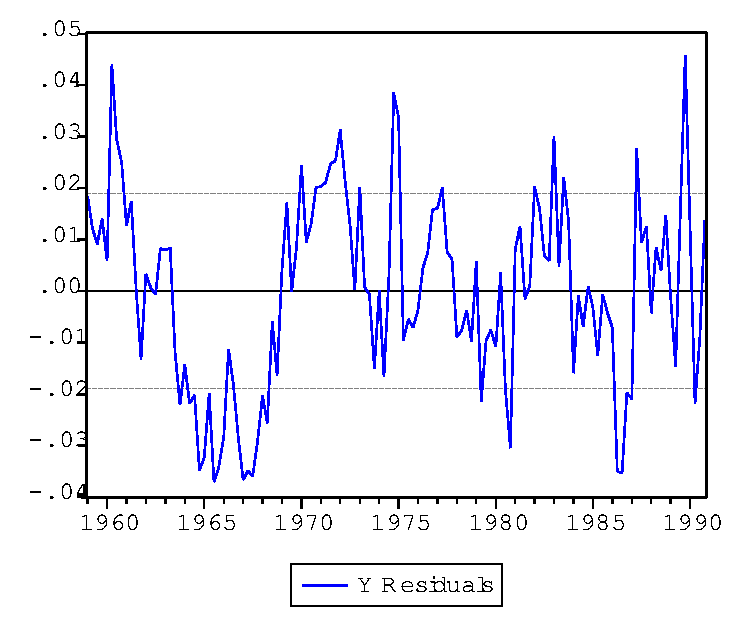
\includegraphics[scale=0.5,angle=0]{graph}
                    \caption{Estimated residuals from model XXX. ...}
                    \label{Fig:Resids}
                \end{center}
                \end{figure}

            \item Tables and graphics may appear in the text or in the appendix, especially if there are many simulation result tabulated, but is also depends on the study and number of tables resp.figures. The key graphs and tables must appear in the text!
        \end{itemize}
 \end{itemize}   
\subsubsection{Instrumental Variable: Hyerin}
Since the fixed effects estimation does not necessarily examine the causal effect of income on democracy, we need a instrumental variable to estimate the causal relation betweem them.    
	\begin{table}[h!] 
		\centering
		\begin{adjustbox}{max width=\textwidth}
		\begin{threeparttable}
			\caption{\textsc{fixed effects results using freedom house measure of democracy: Two-stage least squares with savings rate instrument}}			
			\begin{tabular}{lcccccccc}
		    \hline\hline
		    \ &\multicolumn{8}{c}{Base sample, 1960-2000}\\
		    \cline{2-9}
		    \ &\multicolumn{8}{c}{All countries}\\
		    \cline{2-9}
		    &Pooled &Fixed effects &Fixed effects &Fixed effects &Fixed effects &Fixed effects &Fixed effects &Fixed effects\\[-1.8ex] 	
		    &OLS &OLS &OLS &2SLS &2SLS &2SLS &2SLS &2SLS\\[-1.8ex] 
		    &(1) &(2) &(3) &(4) &(5) &(6) &(7) &(8)\\
		    \hline 
			Panel A &\multicolumn{8}{c}{\textit{Dependent variable is democracy}}\\			
			\hline
			Democracy${}_{t-1}$ &  &  & 0.359 &  & 0.363 &  &  &\\[-1.8ex] 
				&  &  &(0.054) &  & (0.056) &  &  &  \\ 
			Log GDP per capita${}_{t-1}$ & 0.233$^{***}$ & 0.044 & 0.009 & -0.035 & -0.020 & -0.036 & -0.074 & 0.016 \\[-1.8ex] 
				& (0.013) & (0.051) & (0.038) & (0.094) & (0.081) & (0.191) & (0.113) & (0.095) \\ 
			Labor share${}_{t-1}$ &  &  &  &  &  & 0.250 &  &  \\[-1.8ex] 
				&  &  &  &  &  & (0.199) &  &  \\
			\hline
			Panel B &\multicolumn{8}{c}{\textit{First stage for log GDP per capita$_{t-1}$}}\\
			\hline			
			Democracy${}_{t-1}$ &  &  &  &  & 0.144$^{**}$ &  & [0.24] &  \\[-1.8ex] 
				&  &  &  &  & (0.066) &  &  &  \\ 
			Labor share${}_{t-1}$ &  &  &  &  &  & 0.329$^{*}$ &  &  \\[-1.8ex] 
				&  &  &  &  &  & (0.187) &  &  \\ 
			Savings rate${}_{t-2}$ &  &  &  & 1.356$^{***}$ & 1.343$^{***}$ & 1.202$^{***}$ & 1.173$^{***}$ & 1.022$^{***}$ \\[-1.8ex] 
				&  &  &  & (0.277) & (0.270) & (0.315) & (0.254) & (0.218) \\ 
			Savings rate${}_{t-3}$ &  &  &  &  &  &  &  & 0.720$^{***}$ \\[-1.8ex] 
				&  &  &  &  &  &  &  & (0.182) \\ 
				Observations &\multicolumn{1}{c}{891} & \multicolumn{1}{c}{900} & \multicolumn{1}{c}{766} & \multicolumn{1}{c}{900} & \multicolumn{1}{c}{891} & \multicolumn{1}{c}{471} & \multicolumn{1}{c}{733} & \multicolumn{1}{c}{796} \\ 
				R$^{2}$ &\multicolumn{1}{c}{0.226} & \multicolumn{1}{c}{0.115} & \multicolumn{1}{c}{0.225} & \multicolumn{1}{c}{0.571} & \multicolumn{1}{c}{0.571} & \multicolumn{1}{c}{0.725} & \multicolumn{1}{c}{0.541} & \multicolumn{1}{c}{0.536} \\ 
				\hline
			\end{tabular}
		    \begin{tablenotes}
		    	\item \textit{Notes:} This table summarizes the codefficients of each cross-sectional regression. All regression model includes year dummies to capture country-invariant factors. Except for column 1, country dummies are included in the regressions. The robust standrad errors clustered by country are summarized in parentheses. 
		    	\item \begin{align}
		    	^{***}& \text{Significant at the 1 percent level}\notag\\
		    	^{**}& \text{Significant at the 5 percent level}\notag\\
		    	^{*}& \text{Significant at the 10 percent level}\notag
		    	\end{align}
		    \end{tablenotes}
		\end{threeparttable}
		\end{adjustbox}			
	\end{table} 	


\newpage
\subsection{Robustness Tests: Sharon}
\begin{table}[h!] \centering
	\begin{adjustbox}{max width=\textwidth}
		\begin{threeparttable}
			\caption{\textsc{Fixed effects results with alternative samples and additional control variables}}			
			\begin{tabular}{l*{6}{c}} 
			\hline\hline
			& \multicolumn{6}{c}{Five-year data}\\
            \cline{2-7}
			&Balanced panel &&Base sample, 1960-2000, &&&\\[-1.8ex] 
			&1970-2000 &&without former socialist countries  & &\multicolumn{2}{c}{Base sample, 1960-2000}\\
			\cline{2-2} \cline{4-4} \cline{6-7} 
			&Fixed effects &&Fixed effects &&Fixed effects &Fixed effects \\[-1.8ex] 	
			&OLS &&OLS &&OLS&OLS \\[-1.8ex] 			 
&\multicolumn{1}{c}{(1)} &&\multicolumn{1}{c}{(2)} &&\multicolumn{1}{c}{(3)}&\multicolumn{1}{c}{(4)} \\ 
\hline				
&\multicolumn{6}{c}{\textit{Dependent variable is democracy}}\\	
\cline{2-7}	
Democracy$_{t-1}$ & 0.283$^{***}$ && 0.362$^{***}$ && 0.353$^{***}$ & 0.351$^{***}$ \\ [-1.8ex]
& (0.058) && (0.052) && (0.053) & (0.055) \\ 
Log GDP per capita$_{t-1}$ & -0.031 && 0.005 && 0.015 & -0.001 \\ 
& (0.049) && (0.035) && (0.041) & (0.049) \\[-1.8ex] 
Log population$_{t-1}$ &  &&  && -0.109 & -0.042 \\ 
&  &&  && (0.100) & (0.108) \\ 
Education$_{t-1}$ &  &&  &&  & -0.007 \\ [-1.8ex]
&  &&  &&  & (0.020) \\ 
Age Structure$_{t-1}$ &  &&  && [0.05] & [0.19] \\
Observations & \multicolumn{1}{c}{630} && \multicolumn{1}{c}{908} && \multicolumn{1}{c}{863} & \multicolumn{1}{c}{676} \\[-1.8ex]
Countries &90 &&128 &&142 &95\\[-1.8ex] 
R$^{2}$ & \multicolumn{1}{c}{0.215} && \multicolumn{1}{c}{0.221} && \multicolumn{1}{c}{0.241} & \multicolumn{1}{c}{0.235} \\ 
\hline
\end{tabular}
\begin{tablenotes}
	\item \textit{Notes:} 
\end{tablenotes}
\end{threeparttable}	
\end{adjustbox}
\end{table}

\begin{table}[h] \centering
	\begin{adjustbox}{max width=\textwidth}
		\begin{threeparttable}
			\caption{\textsc{fixed effects results using an alternative dependent variable: polity measure}}			
			\begin{tabular}{l*{7}{c}} 
				\hline\hline
				& \multicolumn{7}{c}{Base sample, 1960-2000}\\
				\cline{2-8}
				& & &&& & &Twenty-year\\[-1.8ex]
				& \multicolumn{3}{c}{Five-year data} && \multicolumn{1}{c}{Ten-year data} && \multicolumn{1}{c}{data}\\
				\cline{2-4}\cline{6-6}\cline{8-8}	
				&Pooled &Fixed effects &Fixed effects &&Fixed effects &&Fixed effects \\[-1.8ex] 	
				&OLS &OLS &OLS &&OLS &&OLS \\[-1.8ex] 			 
				&\multicolumn{1}{c}{(1)} &\multicolumn{1}{c}{(2)} &\multicolumn{1}{c}{(3)} &&\multicolumn{1}{c}{(4)} &&\multicolumn{1}{c}{(5)}\\ 
				\hline 
				Democracy${}_{t-1}$ & 0.749$^{***}$ & 0.449$^{***}$ &  && 0.060 && -0.516$^{***}$ \\[-1.8ex]
				& (0.034) & (0.063) &  && (0.091) && (0.165) \\ 
				Log GDP per capita${}_{t-1}$ & 0.053$^{***}$ & -0.006 & -0.011 && 0.007 && -0.126 \\[-1.8ex] 
				& (0.010) & (0.039) & (0.055) && (0.070) && (0.164) \\ 
				Observations & \multicolumn{1}{c}{854} & \multicolumn{1}{c}{854} & \multicolumn{1}{c}{880} && \multicolumn{1}{c}{419} && \multicolumn{1}{c}{168} \\ 
				R$^{2}$ & \multicolumn{1}{c}{0.772} & \multicolumn{1}{c}{0.396} & \multicolumn{1}{c}{0.248} && \multicolumn{1}{c}{0.257} && \multicolumn{1}{c}{0.544} \\
				\hline 
			\end{tabular}
			\begin{tablenotes}
				\item \textit{Notes:} 
			\end{tablenotes}
		\end{threeparttable}	
	\end{adjustbox}
\end{table}
\begin{itemize}
    \item Discuss results:
        \begin{itemize}
            \item Do the results support or do they contradict economic theory ?
            \item What does the reader learn from the results?
            \item Try to give an intuition for your results.
            \item Provide robustness checks.
            \item Compare to previous research.
        \end{itemize}
\end{itemize}
